\chapter{Mathematical Model}
This chapter presents the foundational relationships of continuum dynamics that are essential for this study. We introduce the governing equations for fluid flow in an unbounded domain, along with a discussion of turbulence and Reynolds decomposition. Additionally, we cover specific characteristics pertinent to modeling blood flow in vessels and summarize the assumptions made in developing the mathematical model employed herein.

\section{Fluid Dynamics}
In this work, we model the fluid as a continuum, treating it as an idealized continuous medium. The governing equations for continuum dynamics derive from the fundamental conservation laws of mass, momentum, and energy, intrinsically linked with the physical properties of the fluid and its surroundings.

Assuming an isolated, isothermal system, the evolution of the fluid flow in three-dimensional space is governed by the following system of partial differential equations:
\begin{subequations}\label{NS}
	\begin{gather}
		\label{a}
		\frac{\partial \rho}{\partial t} + \nabla \cdot (\rho \vec{u}) = 0, \\[5pt]
		\label{b}
		\frac{\partial (\rho \vec{u})}{\partial t} + \nabla \cdot (\rho \vec{u} \otimes \vec{u}) = \nabla \cdot \mathbf{T} + \rho \vec{g},
	\end{gather}
\end{subequations}
where $ \otimes $ denotes the outer product, defined component-wise as $ (\vec{u} \otimes \vec{u})_{ij} = u_{i} u_{j}, \: i,j \in \{1,2,3\} $ \cite{Anderson}. The quantities in \eqref{NS} are defined as follows:
\begin{itemize}
	\item[]{\makebox[3cm]{$ \rho $ \si{[kg.m^{-3}]} \hfill} density of the fluid},
	\item[]{\makebox[3cm]{$ \vec{u} $ \si{[m.s^{-1}]} \hfill} vector of macroscopic velocity,}
	\item[]{\makebox[3cm]{$ \mathbf{T} $ \si{[kg.m^{-1}.s^{-2}]} \hfill} total stress tensor,}
	\item[]{\makebox[3cm]{$ \vec{g} $ \si{[m.s^{-2}]} \hfill} vector of external force accelerations.}
\end{itemize}
Each of these quantities is generally a function of time $ t $ \si{[s]} and spatial position $ \vec{x} $ \si{[m]}.

For an isothermal system, the ideal gas equation of state applies, expressed as:
\begin{equation}\label{pressure}
	p = c^{2}_{s} \ \rho,
\end{equation}
where $ p $ \si{[Pa]} represents the pressure, and $ c_{s} $ \si{[m.s^{-1}]} is the speed of sound in the fluid \cite{Latt}. Together, equations \eqref{NS} and \eqref{pressure} form a closed system, allowing the model to omit the energy conservation law.

\subsection{Stress Tensor}

We denote the dynamic stress tensor as $\mathbf{T}_{\mu} = \big(\sigma^{\, \mu}_{ij} \big)$ \si{[kg.m^{-1}.s^{-2}]}, where $i,j \in \{1,2,3\}$. For Newtonian fluids, each component of the dynamic stress tensor linearly depends on the spatial velocity derivatives. Fluids that do not satisfy this linear relationship are classified as non-Newtonian. For Newtonian fluids, the dynamic stress tensor components are given by \cite{Schlichting}:

\begin{subequations}\label{newton}
	\begin{eqnarray}
		\sigma^{\, \mu}_{ii} = \lambda \nabla \cdot \vec{u} + 2 \mu \frac{\partial u_i}{\partial x_i},&& \hspace{-3mm} i \in \{1,2,3\}, \\[5pt]
		\sigma^{\, \mu}_{ij} = \sigma^{\, \mu}_{ji} = \mu \left( \frac{\partial u_i}{\partial x_j} + \frac{\partial u_j}{\partial x_i} \right),&& \hspace{-4mm} \ i,j \in \{1,2,3\}, \: i \neq j,
	\end{eqnarray}
\end{subequations}
where $ \mu $ \si{[kg.m^{-1}.s^{-1}]} is the dynamic viscosity, and $ \lambda $ \si{[kg.m^{-1}.s^{-1}]} represents the second viscosity coefficient~\cite{Cengel}. For Newtonian fluids, $\mathbf{T}_{\mu}$ is symmetric by definition.

By introducing the strain rate tensor~$\mathbf{D}$ \si{[s^{-1}]}, defined as
\begin{equation}\label{eq:D}
	\mathbf{D} = \frac{1}{2} \left[ \nabla \vec{u} + (\nabla \vec{u})^T \right],
\end{equation}
the dynamic stress tensor can be equivalently expressed as
\begin{equation}\label{eq:1}
	\mathbf{T}_{\mu} = 2 \mu \mathbf{D} + \left( \lambda + \frac{2}{3} \mu \right) (\nabla \cdot \vec{u}) \mathbf{I},
\end{equation}
where $ \mathbf{I} $ denotes the identity tensor in three-dimensional space. By invoking Stokes' hypothesis, which states $ \lambda = -\frac{2}{3} \mu $ \cite{Anderson}, the above equation simplifies to
\begin{equation}
	\mathbf{T}_{\mu} = 2 \mu \mathbf{D}.
\end{equation}
The complete stress tensor for a Newtonian fluid is then given by
\begin{equation}\label{eq:T}
	\mathbf{T} = -p\mathbf{I} + \mathbf{T}_{\mu},
\end{equation}
where $ \mathbf{I} $ remains the identity tensor in three-dimensional space \cite{Cengel}.

The strain rate tensor also facilitates defining the shear rate $ \dot{\gamma} $~\si{[s^{-1}]} \cite{Cengel} as
\begin{equation}\label{eq:dot gamma}
	\dot{\gamma} = \sqrt{2} \| \mathbf{D} \| _{F},
\end{equation}
where $ \| \cdot \| _{F} $ denotes the Frobenius norm, defined for a matrix $ \mathbf{A} $ of dimensions $ m \times n $ with elements $ a_{ij} $ as
\begin{equation}
	\| \mathbf{A} \| _{F}  \coloneqq \sqrt{\sum_{i = 1}^{m} \sum_{j = 1}^{n} |a_{ij}|^2}.
\end{equation}

To characterize fluid interaction with boundaries, the wall shear stress, denoted by $ \tau _w $ \si{[kg.m^{-1}.s^{-2}]} and commonly referred to as the \textit{wall shear stress} \cite{WallStress}, is often used. In three-dimensional space, it is defined by
\begin{equation}\label{eq:wall shear stress}
	\tau_w = \mathbf{T} \cdot \vec{t},
\end{equation}
where $ \vec{t} $ is the unit tangent vector at the wall at the given point.

\subsection{Turbulence and Reynolds Decomposition}\label{turb}
We define turbulent flow as a flow state that is disordered in both time and space, characterized by continuous fluctuations in both the direction and magnitude of velocity. This results in random, unstable behavior that distinguishes turbulence from laminar flow.

Turbulence typically occurs at high values of the Reynolds number, a dimensionless parameter defined by
\begin{equation}\label{Re}
	\mathrm{Re} = \dfrac{l_{0} u_{0}}{\nu} = \dfrac{l^{2}_{0}}{t_{0} \nu},
\end{equation}
where $ \nu $ represents the kinematic viscosity \si{[m^2.s^{-1}]}, and $ l_{0} $~\si{[m]}, $ t_{0} $~\si{[s]}, and $ u_{0} $~\si{[m.s^{-1}]} denote the characteristic length, time, and velocity relevant to the specific flow \cite{Landau}.

Due to the complex and stochastic nature of turbulent flow, its precise description is inherently challenging. A common approach is to employ Reynolds' time-averaging method, where the instantaneous value of a flow variable $ \psi $ is decomposed into its mean value $ \overline{\psi} $ and a fluctuating component $ \psi' $:
\begin{equation}
	\psi = \overline{\psi} + \psi'.
\end{equation}
Here, the fluctuation $ \psi' $ is defined such that its time-averaged value over a sufficiently long period is zero, i.e., $ \overline{\psi'} = 0 $ \cite{Schlichting}.

In this decomposition, $ \psi $ can represent any scalar quantity, such as the components of velocity $ \vec{u}_i $, pressure $ p $, or density $ \rho $ \cite{Sodja2007}. The averaging period should be significantly larger than the time scale of the turbulent fluctuations being studied, ensuring that the mean values accurately represent the underlying flow structure \cite{Sodja2007}.

Focusing on the Reynolds decomposition of the velocity field $ \vec{u} (\vec{x}, t) $ with respect to time averaging, we define the turbulent kinetic energy $ T_{\text{turb}} $~\si{[m^{2}.s^{-2}]} as
\begin{equation}\label{eq:turb kin energy}
	T_{\text{turb}} = \dfrac{1}{2} \left( \overline{(u_1 ')^2} + \overline{(u_2 ')^2} + \overline{(u_3 ')^2} \right) = \dfrac{1}{2} \overline{ \left( u_1 '^2 + u_2 '^2 + u_3 '^2 \right) },
\end{equation}
where we utilize the arithmetic properties of Reynolds decomposition to obtain this expression \cite{Sodja2007}.

\section{Description of Vascular Flow}\label{cevni proudeni}
Due to the presence of numerous physical, chemical, and physiological processes, vascular flow represents a highly complex process. In many cases, however, a simplified model that neglects some characteristics suffices for its description \cite{Saloner2019}. In this section, we briefly describe some aspects for which a simplified model can be considered under appropriate assumptions.

\section*{\fontsize{11}{15}\selectfont Elasticity of Walls}
The interaction of an elastic body, i.e., a body with a movable boundary, can be modeled, for example, using the immersed boundary method \cite{Peskin}. In many cases, however, the elasticity of wall obstacles can be neglected, and only rigid geometry considered. Particularly in smaller vessels, neglecting the elasticity of the vascular walls has not shown a significant effect on the outcome. \cite{DempereMarco2006} However, this is not always the case, as significant non-negligible effects on the overall error of the results have been observed in the area of the aorta when considering rigid geometry. \cite{LANTZ2011}

Note that including the elasticity of vascular walls in the considered model requires appropriately defining the conditions of interaction with the fluid, which is generally a difficult task in vascular flow, often depending on the correct evaluation of \textit{in vivo} measurements. Additionally, in diseases such as arteriosclerosis\footnote{Arteriosclerosis is a disease in which the arterial walls thicken and subsequently lose their elasticity \cite{Fishbein2015}.}, vessels lose their elasticity in many patients, thus including elasticity in the model may not necessarily reflect the physiological state of the vessels correctly \cite{Saloner2019}.

\section*{\fontsize{11}{15}\selectfont Blood Viscosity}

For the mathematical model, it is important to choose the viscosity values correctly to encompass any non-Newtonian behavior of the fluid under investigation. Blood is generally considered a Newtonian fluid. However, there are situations where the Newtonian behavior of blood is compromised. For instance, in cases where the flow velocity of blood is very low, red blood cells can accumulate, consequently increasing the viscosity of blood.
Areas with such slow flow can be found, for example, in regions of aneurysmatic dilation\footnote{Aneurysmatic dilation refers to a disease condition where there is a local enlargement of a vessel \cite{Syed1997}.}. On the other hand, the viscosity of blood significantly decreases in areas where blood flows through very narrow vessels, particularly through vessels at the scale of arterioles or capillaries \cite{Saloner2019}.

There are viscosity models that aim to more accurately capture the physical description and behavior of blood viscosity~\cite{Saloner2019, Eichler2023, Boyd2007}. The simplest is the so-called Power-Law model \cite{Sequeira}. The Power-Law model prescribes for viscosity
\begin{equation}\label{eq:power-law}
	\mu _{\text{PL}} (\dot{\gamma}) = K_p  \dot{\gamma} ^{n_1-1} \ ,
\end{equation}
where $ K_p$ \si{[kg.m^{-1}]} and $ n_1 $ \si{[-]} are constants. Another model is the Casson model \cite{Boyd2007} which satisfies
\begin{equation}\label{eq:Casson}
	\mu _{\text{CA}} (\dot{\gamma}) = \frac{1}{\dot{\gamma}} \left[ k_{0} + k_{1} \sqrt{\dot{\gamma}} \right]^2 \ ,
\end{equation}
where $ k_1$ \si{[kg^{2}.m^{-2}]} and $ k_2 $ \si{[kg^{2}.m^{-2}]} are empirically determined constant parameters. A major advantage of these basic models is that for certain geometries and under specific conditions, exact solutions are available, which for example, provide reference values for numerical simulations. An obvious disadvantage of these models is their limited applicability, as they fail for shear rates approaching zero \cite{Boyd2007}.

Among the more complex models, the Cross model \cite{Sequeira} is defined by the relation
\begin{equation}\label{eq:cross}
	\mu _{\text{CR}} (\dot{\gamma}) = \frac{\mu_{0} - \mu_{\infty}}{1 + (k\dot{\gamma})^{n_2}} + \mu_{\infty}  \ ,
\end{equation}
where $ k $ \si{[s]} and $ n_2 $ \si{[-]} are constants, and it is also valid that
\begin{equation}\label{eq:m0 a minf}
	\mu _{0}  = \lim_{\dot{\gamma} \rightarrow 0+}\mu (\dot{\gamma})\, , \ \mu_{\infty} = \lim_{\dot{\gamma} \rightarrow \infty}\mu (\dot{\gamma}).
\end{equation}
The last mentioned model is the Carreau-Yasuda model \cite{Boyd2007} satisfying
\begin{equation}\label{eq:C-Y}
	\mu _{\text{CY}} (\dot{\gamma}) = \mu_{\infty} + (\mu_{0} - \mu_{\infty}) \left[ 1 + (\varepsilon \dot{\gamma}) ^{a} \right]^{\frac{n_3-1}{a}} \ ,
\end{equation}
where $ \varepsilon$ \si{[s]} , $a$ \si{[-]}, and $ n_3 $ \si{[-]} are again empirically determined constant parameters that influence the model behavior between boundary viscosity values. For $ \mu_{0}$ and $ \mu_{\infty} $ the condition \eqref{eq:m0 a minf} still applies.

All mentioned models are compared in Fig. \ref{fig:vs}, with parameter values taken from \cite{Eichler2023}.
\begin{figure}[H]
	\centering
	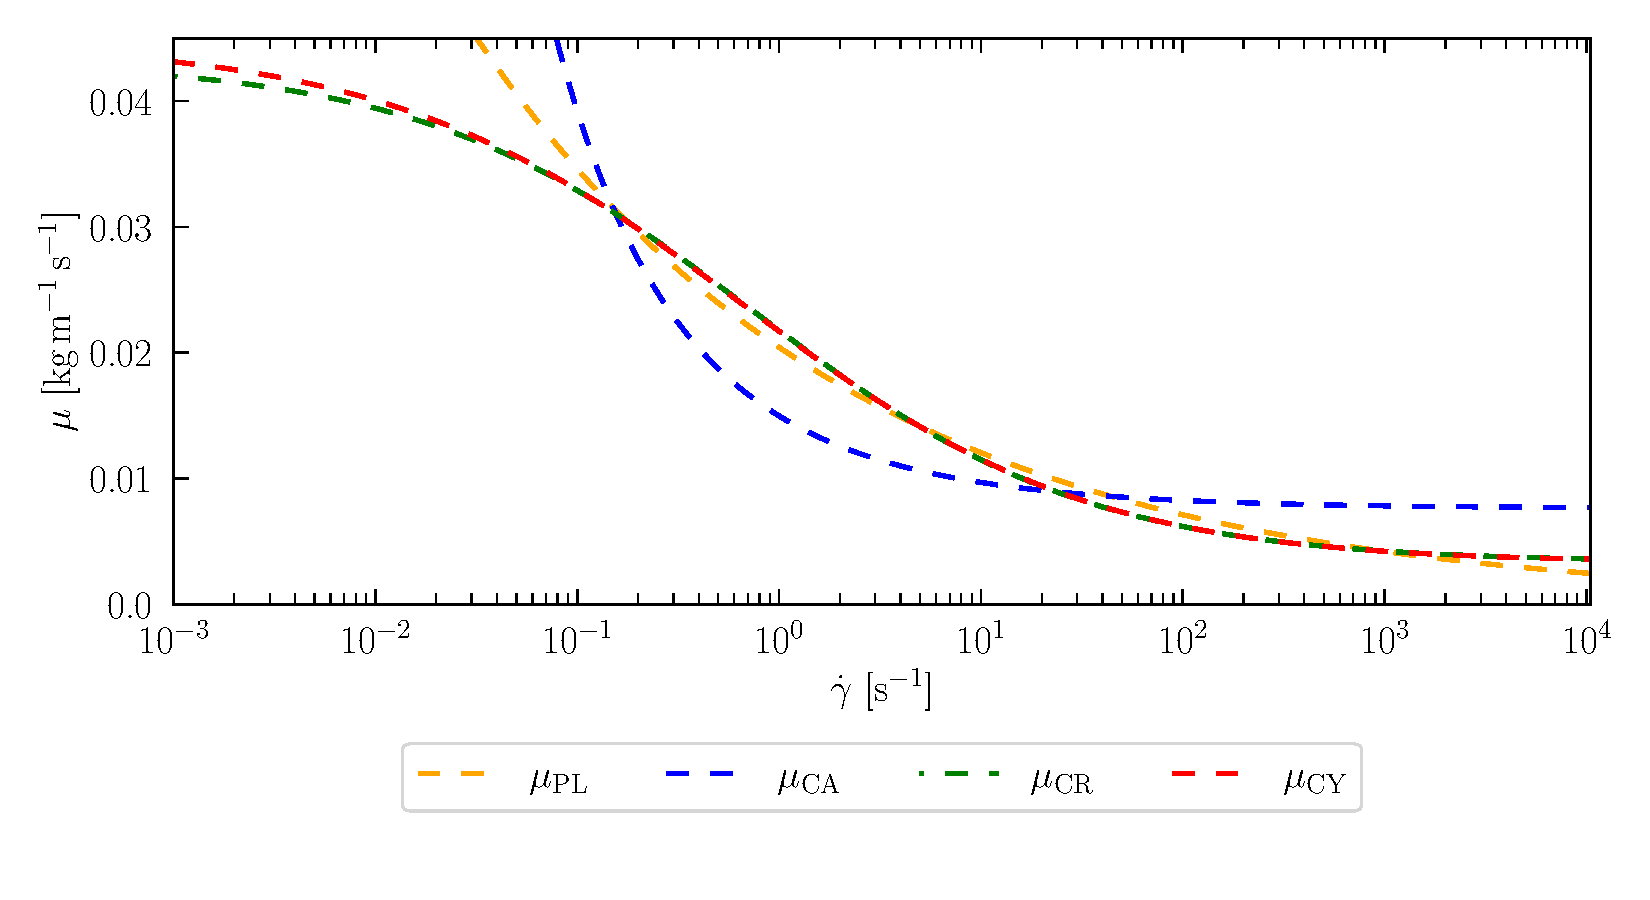
\includegraphics[width=1.0\textwidth]{figures/modely.pdf}
	\vspace{-9mm}
	\caption{Comparison of non-Newtonian viscosity models, specific parameter values were taken from \cite{Eichler2023}. Descriptions of each model correspond to the defining equations
		\eqref{eq:power-law}, \eqref{eq:Casson}, \eqref{eq:cross}, and \eqref{eq:C-Y}.}
	\label{fig:vs}
\end{figure}
We note that in this work, blood will be considered exclusively as a Newtonian fluid.

\section*{\fontsize{11}{15}\selectfont Turbulent Flow}
In most cases, blood flow can be approximated by laminar flow \cite{Sequeira}. However, in some instances in vascular flow, turbulence and chaotic behavior occur \cite{Saqr2020}. One area where turbulence can be observed is behind a vascular stenosis\footnote{Vascular stenosis is a condition in which there is a local narrowing of a vessel \cite{Carabello2009}.} \cite{Jain2022}. The flow velocity of blood in the narrowed area can significantly increase, and the reduction in the diameter of the vessel ensures that the flow remains laminar in this section of the constriction \cite{Sequeira}. However, immediately after the constriction, the flow velocity remains elevated even in areas with the original diameter, which can lead to the formation of vortices and a change in flow regime \cite{Saloner2019, Varghese2003}.

The occurrence of turbulent flow is physiologically undesirable as it is often accompanied by significant dissipation of kinetic energy, which can strain parts of the circulatory system. Additionally, vascular areas with turbulence show increased strain on vessel walls, which can lead to tissue damage and diseases such as arteriosclerosis. Therefore, it is desirable to minimize turbulence in blood flow \cite{Saloner2019, Kameneva2004}.

\section{Assumptions of the Mathematical Model in This Work}\label{pred}
In this section, we summarize the additional assumptions applied to our system to simplify solving the governing equations \eqref{NS}. Specifically, we assume an isothermal system (i.e., constant temperature over time) with no external forces acting on it. The fluid under consideration is incompressible, Newtonian, and characterized by a constant dynamic viscosity.

We consider a rectangular domain $ \Omega \subset \mathbb{R}^3 $, defined by $ \Omega = (0, L_1) \times (0, L_2) \times (0, L_3) $, where $ L_1 $, $ L_2 $, and $ L_3 $ \si{[m]} represent the domain dimensions along each spatial axis. The temporal interval is denoted by $ \mathcal{I} = \langle 0, T \rangle $, where $ T > 0 $. With these assumptions, the governing equations \eqref{NS} on $ \Omega \times \mathcal{I} $ simplify to \cite{Schlichting}:

\begin{subequations}\label{NS s predpoklady}
	\begin{gather}
		\label{a s predpoklady}
		\nabla \cdot \vec{u} = 0, \\[5pt]
		\label{b s predpoklady}
		\rho \frac{\text{D} \vec{u}}{\text{D} t} = - \nabla p + \mu \Delta \vec{u},
	\end{gather}
\end{subequations}
where we have introduced the material derivative operator
\begin{equation}
	\dfrac{\text{D}}{\text{D} t} \coloneqq \dfrac{\partial}{\partial t} + \vec{u} \cdot \nabla.
\end{equation}

The boundary of $ \Omega $ is partitioned as follows: $ \partial \Omega_{\text{in}} $ denotes the inflow boundary where inlet conditions are specified; $ \partial \Omega_{\text{out}} $ represents the outflow boundary; and $ \partial \Omega_{\text{w}} $ corresponds to the wall boundaries, where a no-slip condition is imposed. The system \eqref{NS s predpoklady} is supplemented by the following initial and boundary conditions:

\begin{subequations}\label{eq:okrajovky}
	\begin{alignat}{3}
		&\vec{u} = \vec{u}_{\text{ini}},  &p = p_{\text{ini}} \hspace{5mm} &\text{on } \ \Omega \times \mathcal{I},\\[3pt]
		&(\nabla p - \nu \Delta \vec{u}) \cdot \vec{n}  = 0, &\vec{u} = \vec{u}_{\text{in}} \hspace{5mm} &\text{on } \ \partial \Omega_{\text{in}} \times \mathcal{I},\\[3pt]
		&\vec{u} = \vec{0}, \, &\nabla p \cdot \vec{n} = 0 \hspace{5mm} &\text{on } \ \partial \Omega_{\text{w}} \times \mathcal{I},\\[3pt]
		&p = p_{\text{out}}, &\nabla u_i \cdot \vec{n} = 0 \hspace{5mm} &\text{on } \ \partial \Omega_{\text{out}} \times \mathcal{I}, \quad i = 1, 2, 3,
	\end{alignat}
\end{subequations}
where $ \vec{n} $ is the outward-pointing normal unit vector to the boundary $ \partial \Omega $. Here, $ \vec{u}_{\text{ini}}$ \si{[m.s^{-1}]} and $ p_{\text{ini}} $ \si{[kg.m^{-1}.s^{-2}]} denote the initial velocity and pressure, respectively; $ \vec{u}_{\text{in}}$ \si{[m.s^{-1}]} is the prescribed inflow velocity at $ \partial \Omega_{\text{in}} $; and $ p_{\text{out}} $~\si{[kg.m^{-1}.s^{-2}]} is the prescribed outflow pressure at $ \partial \Omega_{\text{out}} $. Initial and boundary conditions are further elaborated in Section~\ref{pocatecni a okrajove podminky}.

